\documentclass{article}
\usepackage{amsmath}
\usepackage{amssymb}
\usepackage{graphicx}
\usepackage{bbm}
\newcommand
\bbone{\ensuremath{\mathbbm{1}}}

\author{Yichen ZHU}
\title{SIGMA203b Mini Projet}
\begin{document}
\maketitle

\section{Questions lab}

\subsection{Exercice 1. D\'ebruitage et interpolation sinusoidal avec Filtre Kalman}
\subsubsection{G\'en\'eration des donn\'ees}
On a un mod\`ele HMM qui repr\'esente la phase d'un signal sinusoidal :
\[
\begin{array}{r c l}
X_{0} &=& X_{0} \sim \mathcal{N}(0,S) \\
X_{t}|X_{t-1} &=& x_{t-1} \sim \mathcal{N}(Ax_{t-1},Q) \\
Y_{t}|X_{t} &=& x_{t} \sim \mathcal{N}(Bx_{t},R) \\
A &=& exp(-\gamma)\begin{pmatrix}
								\cos(\omega) & -\sin(\omega) \\
								\sin(\omega) & \cos(\omega)
								\end{pmatrix} \\
B &=& \begin{pmatrix}
		\sqrt{2} & 0
		\end{pmatrix}
\end{array}
\]
\begin{figure}[!h]
\begin{center}
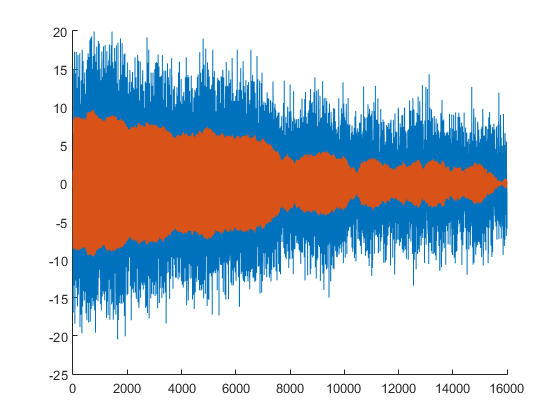
\includegraphics[scale=0.5]{ex1_gd.png}
\end{center}
\caption{Observation en bleu et vrai etat en rouge}
\end{figure}
On g\'en\`ere $X$ et $Y$ selon ce mod\`ele en utilisant la fonction $lingauss\_simul$ et on s'int\'eresse aux param\`etres $\omega$,$\gamma$,$Q$ et $R$. $\omega$ est donc le param\`etre de fr\'equence et $\gamma$ permet de faire d\'ecroitre l'energie ou autrement dit l'amplitude du signal. Plus $\gamma$ est grand, plus vite l'energie d\'ecroit. $Q$ est le bruit d'\'evolution quand il est grand, la variance c'est \`a dire l'incertitude de $X$ est grand. $R$ est le bruit d'observation, on observe $X$ avec un bruit, plus l'observation est bruit\'ee, moins le r\'esultat est pr\'ecis.

\subsubsection{D\'ebruitage}
On impl\'emente le filtre Kalman pour d\'ebruiter l'observation et estimer $X$. Le principe de cette m\'ethode est de prendre la moyenne de la pr\'ediction et l'observation comme si on a deux mesures pour pr\'eciser la valeur estim\'ee. 
\begin{figure}[h]
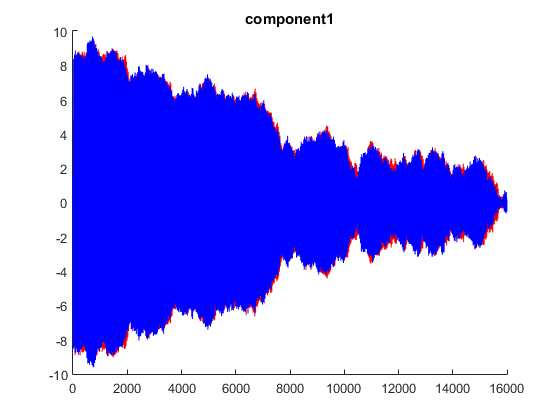
\includegraphics[scale=0.25]{ex1_kf1.png} 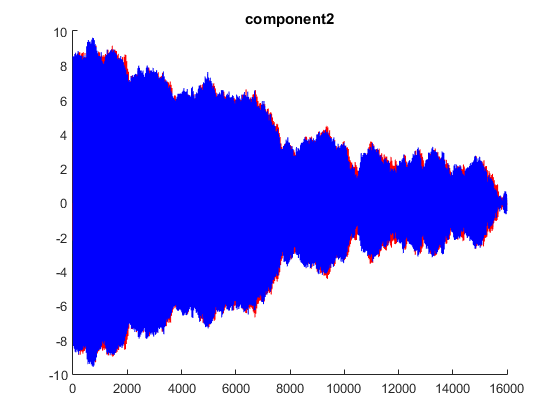
\includegraphics[scale=0.25]{ex1_kf2.png} 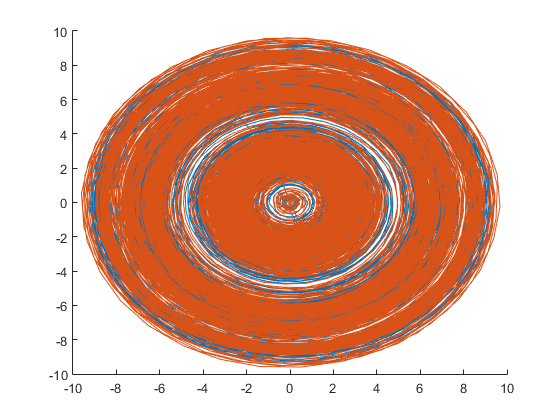
\includegraphics[scale=0.25]{ex1_kf3.png} 
\caption{Projection du signal sur trois axes}
\end{figure} \\
Quand on fait augmenter le bruit d'observation, on calcule le SNR pour evaluer l'efficacit\'e du filtre Kalman. Il n'y a pas beaucoup de diff\'erence pour le SNR quand R est dans l'ordre de $10^{4}$. Cela prouve que le filtre Kalman est tr\`es utile pour des observations bruit\'ees.
\subsubsection{R\'estauration}
On veut montrer que m\^eme si l'observation $Y$ n'est pas compl\`ete, le filtrage fonctionne toujours. Cela vient du fait que :
\[
p(x_{k+1}|x_{k}) = \int p(x_{k+1}|x_{k}) p(x_{k}|y_{1:k}) dx_{k}
\]
On met une partie de $y$ en $0$ : \\
\begin{figure}[!h]
\begin{center}
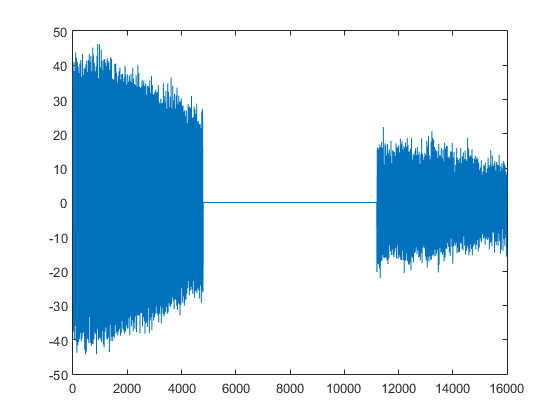
\includegraphics[scale=0.25]{ex1_rstY.png}
\end{center}
\caption{Observation n'est pas compl\`ete}
\end{figure} \\
on applique le filtre de Kalman : \\
\begin{figure}[!h]
\begin{center}
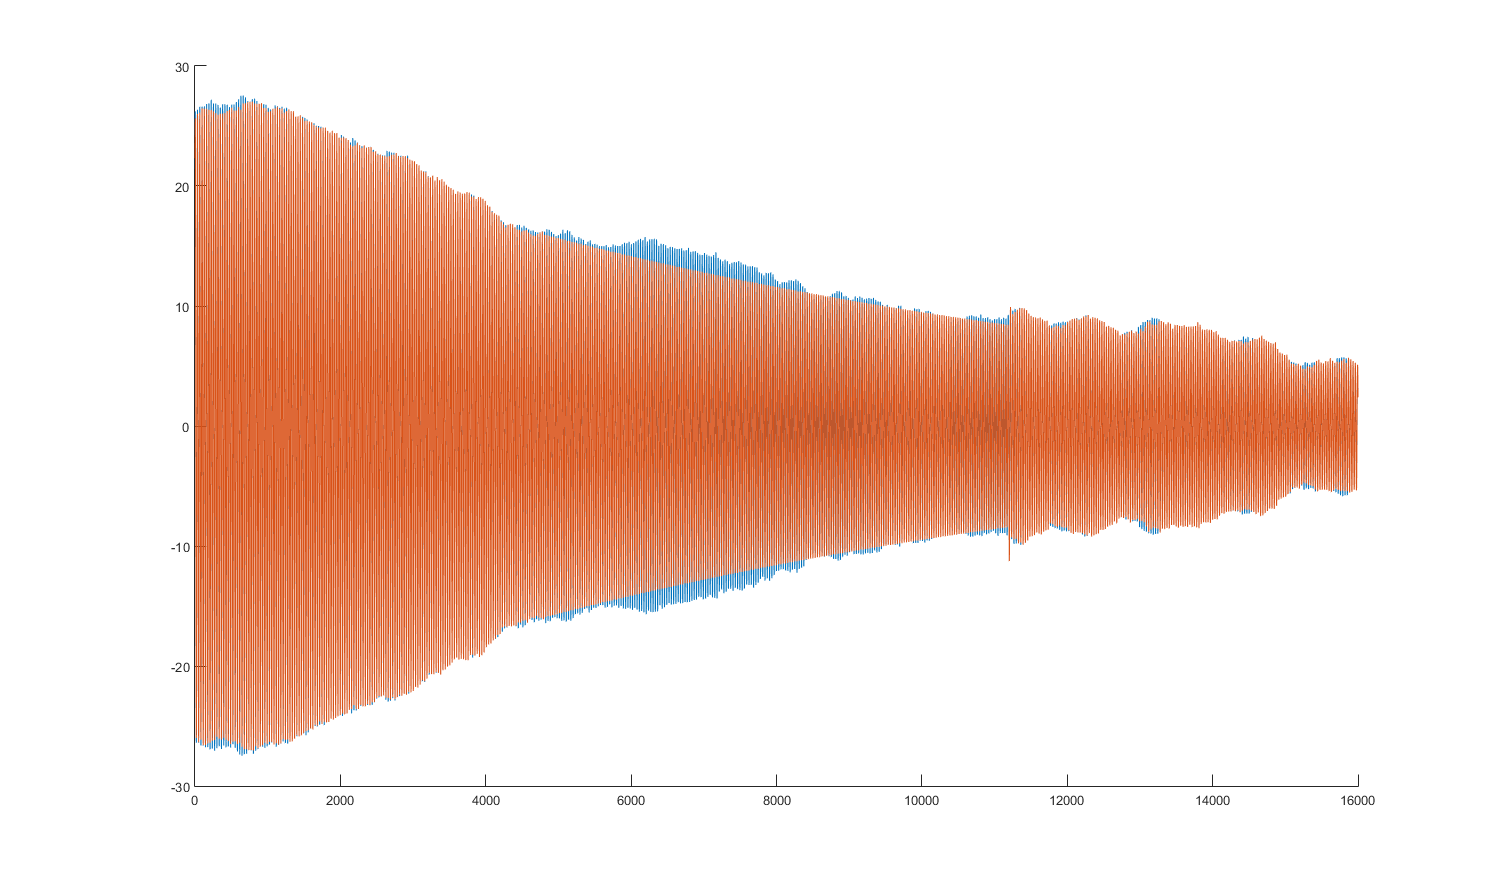
\includegraphics[scale=0.2]{ex1_rst.png}
\end{center}
\caption{Vrai etat en bleu et estim\'e en rouge}
\end{figure} \\
Donc on voit qu'en utilisant la pr\'ediction, l'absence de $B$ n'est pas un probl\`eme pour restaurer la partie perdue.
\subsection{Exercice 2. Pitch tracking monophonique avec Filtre Particulaire}
\subsubsection{G\'en\'eration des donn\'ees}
On prend toujours le m\^eme mod\`ele pour g\'en\'erer le sinus, on rajoute encore un \'etat cach\'e pour la fr\'equence. Donc on a $M$ pitch \`a utiliser. La matrice de transition pour aller d'un pitch \`a un autre est (ici on prend $M=3$) :
\[
p(R_{t}|R_{t-1}) = \begin{pmatrix}
									 1-\nu & \frac{\nu}{M-1} & \frac{\nu}{M-1} \\
									 \frac{\nu}{M-1} & 1-\nu & \frac{\nu}{M-1} \\
									 \frac{\nu}{M-1} & \frac{\nu}{M-1} & 1-\nu
									 \end{pmatrix}
\]
On g\'en\`ere une m\'elodie et on l'\'ecoute :
\begin{figure}[!h]
\begin{center}
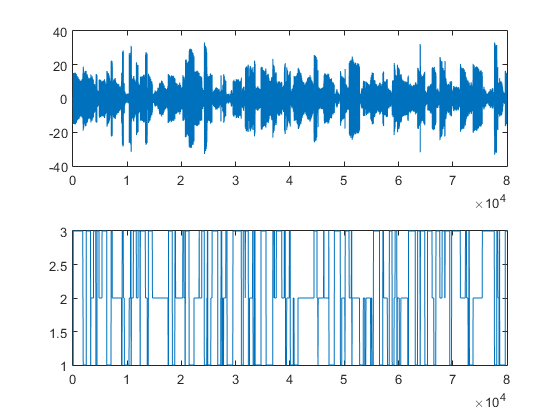
\includegraphics[scale=0.25]{ex2_gd.png}
\end{center}
\caption{G\'en\'eration des donn\'ees}
\end{figure} \\
\subsubsection{Pitch tracking}
On impl\'emente l'algorithme du SIS (Sequential Importance Sampling). Ici on utilise le Bootstrap Filter c'est \`a dire que notre loi de proposition :
\[
\pi(X_{k}|X_{0:k-1},y_{1:k}) = p(X_{k}|X_{k-1}) 
\]
\`A chaque instant, on tire $N$ \'echantillons qui suivent la loi de proposition $\pi$. Comme c'est un Bootstrap filtre, on fait evoluer le poid $W$ avec la loi d'observation $p(Y_{k}|X_{k})$ et on note $W^{*}=Wp(Y_{k}|X_{k})$. Quand on finit de tirer les particules, on pose $W = \frac{W^{*}}{\sum W^{*}}$.
Ici ce qu'on veut estimer est l'indice du pitch $r$, \`a la fin de chaque tirage, on prend le maximum du poid $W$ pour voir quelle est la particule la plus importante. On fait it\'erer cet algorithme et on a le r\'esultat :
\begin{figure}[!h]
\begin{center}
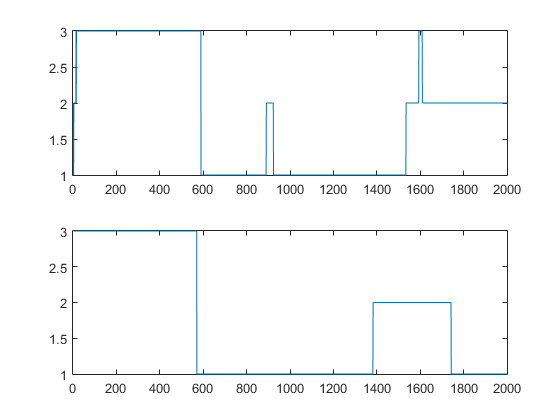
\includegraphics[scale=0.4]{ex2_fp2.png}
\end{center}
\caption{etat estim\'e et vrai etat}
\end{figure} \\

\section{Questions \'ecrites}

\subsection{Exercice 3. Filtre de Kalman \'etendu}
\subsubsection{Calcul des diff\'erentielles} On a notre mod\`ele HMM :
\[
\left\{
\begin{array}{r c l}
\left(
\begin{array}{r c l}
X_{1,k+1}\\
X_{2,k+1}
\end{array}
\right)                &=&  \left(
													\begin{array}{r c l}
													X_{1,k+1} + hX_{2,k+1}\\
													X_{2,k+1} -\gamma h \sin(X_{1,k+1})
													\end{array}
													\right) + \left(
																		\begin{array}{r c l}
																		\epsilon_{1,k+1}\\
																		\epsilon_{2,k+1}
																		\end{array}
																		\right)\\
																		
Y_{k+1} &=& \sin(X_{1,k+1}) + \eta_{k+1}
\end{array}
\right.
\]
On r\'eecrit le mod\`ele avec les fonctions $f,g$ sous la forme ci-dessous :
\[
\left\{
\begin{array}{r c l}
X_{k+1} &=& f(X_{k}) + \epsilon_{k} \\
Y_{k+1} &=& g(X_{k+1}) + \eta_{k+1}
\end{array}
\right.
\]
avec : 
\[
\left\{
\begin{array}{r c l}
f(X_{1,k},X_{2,k}) = \left(
													\begin{array}{r c l}
													X_{1,k+1} + hX_{2,k+1}\\
													X_{2,k+1} -\gamma h \sin(X_{1,k+1})
													\end{array}
													\right) \\
g(X_{1,k+1},X_{2,k+1}) = \sin(X_{1,k+1})
\end{array}
\right.
\]
Les fonctions $f,g$ sont non-lin\'eaires, on veut donc effectuer une approximation gaussienne pour lin\'eariser ce mod\`ele. On calcule la diff\'erentielle de $f$ au $X_{k}$ et celle de $g$ au $X_{k+1}$ :
\[
\left\{
\begin{array}{r c l}
F_{x} &=& \begin{pmatrix}                               
								1 & h \\
								-\gamma h \cos(X_{1,k}) & 1 \\
							\end{pmatrix} \\
G_{x} &=& \begin{pmatrix}                               
							\cos(X_{1,k}) & 0 \\
							\end{pmatrix}
\end{array}
\right.
\]
\subsubsection{\'Etape de pr\'ediction} On suppose que $(X_{1,k-1}|y_{1:k-1}) \sim \mathcal{N}(m_{k-1},P_{k-1})$ On en d\'eduit la loi jointe $\left(
				\begin{array}{r c l}
			  X_{k-1} \\
				X_{k}
				\end{array}|y_{1:k-1}
				\right)$ en fonction de $m_{k-1},P_{k-1}$. On a donc :
\[
\mathcal{L}\left(
					 \begin{array}{r c l}
					 X_{k-1} \\
					 X_{k}
					 \end{array}|y_{1:k-1}
			     \right) = \mathcal{L}\left(
										 \begin{array}{r c l}
					           X_{k-1} \\
					           f(X_{k-1}) + \epsilon_{k-1}
					           \end{array}|y_{1:k-1}
			               \right) = \mathcal{L}\begin{pmatrix}
					                                W_{k-1} \\
					                                f(W_{k-1}) +\epsilon_{k-1}
					                                \end{pmatrix}
\]
D'o\`u $W_{k}$ est un vecteur al\'eatoire $W_{k} \sim \mathcal{N}(m_{k-1},P_{k-1})$ Ensuite, on effectue l'approximation lin\'eaire :
\[
					 \begin{pmatrix}
					 m_{k-1} + \delta W_{k-1} \\
					 f(m_{k-1}) + A\delta W_{k-1} +\epsilon_{k-1}
					 \end{pmatrix} \sim \mathcal{N} \left(
					                                \begin{pmatrix}
					                                m_{k-1} \\
					                                m^{-}_{k}
					                                \end{pmatrix} , \begin{pmatrix}
					                                                P_{k-1} & P_{k-1}A^{T}\\
					                                                AP_{k-1} & P^{-}_{k}
					                                                \end{pmatrix}
					                                \right)
\]
Avec : $A$ la diff\'erentielle $A = F_{x}(m_{k-1})$, $m^{-}_{k}=f(m_{1,k-1},m_{2,k-1})$ et $P^{-}_{k}=AP_{k-1}A^{T} +Q_{k-1}$. On peut donc en d\'eduire l'approximation de la loi marginale $\mathcal{L}(X_{k}|y_{1:k-1})\approx\mathcal{N}(m^{-}_{k},P^{-}_{k})$ 																																																		
\subsubsection{\'Etape de mise \`a jours}Pareil que  l'\'etape de pr\'ediction, on fait l'approximation lin\'eaire pour la loi jointe $\left(
					                                                                                                    \begin{array}{r c l}
					                                                                                                    X_{k} \\
					                                                                                                    Y_{k}
					                                                                                                    \end{array}|y_{1:k-1}
			                                                                                                        \right)$ pour effectuer l'\'etape de mise \`a jours. On a donc :
\[
\mathcal{L}\left(
					 \begin{array}{r c l}
					 X_{k} \\
					 Y_{k}
					 \end{array}|y_{1:k-1}
			     \right) = \mathcal{L}\left(
										 \begin{array}{r c l}
					           X_{k} \\
					           g(X_{k}) + \eta_{k}
					           \end{array}|y_{1:k-1}
			               \right) = \mathcal{L}\begin{pmatrix}
					                                W_{k} \\
					                                g(W_{k}) +\eta_{k}
					                                \end{pmatrix}
\]
D'o\`u $W_{k}$ est un vecteur al\'eatoire $W_{k} \sim \mathcal{N}(m^{-}_{k},P^{-}_{k})$. Ensuite, on exprime $\mathcal{L}\begin{pmatrix}
																																																											     W_{k} \\
					                                                                                                                 g(W_{k}) +\eta_{k}
					                                                                                                                 \end{pmatrix}$ en fonction de $m^{-}_{k},P^{-}_{k}$ :
\[
\begin{pmatrix}
					 m^{-}_{k} + \delta W_{k} \\
					 f(m^{-}_{k}) + B\delta W_{k} + \eta_{k}
					 \end{pmatrix} \sim \mathcal{N} \left(
					                                \begin{pmatrix}
					                                m^{-}_{k} \\
					                                g(m^{-}_{k})
					                                \end{pmatrix} , \begin{pmatrix}
					                                                P^{-}_{k} & P^{-}_{k}B^{T}\\
					                                                BP^{-}_{k} & S
					                                                \end{pmatrix}
					                                \right)
\]
Avec : $B$ la diff\'erentielle $B = G_{x}(m^{-}_{k})$ et $S = BP^{-}_{k}B^{T} +R_{k}$.  																																																								
\subsubsection{Filtrage} On en d\'eduit donc l'approximation de la loi marginale de filtrage: $\mathcal{L}(X_{k}|y_{1:k})\approx\mathcal{N}(m_{k},P_{k})$ avec :
\[
\left\{
\begin{array}{r c l}
m_{k} &=& f(m_{1,k-1},m_{2,k-1}) + K(y_{k}-g(f(m_{1,k-1},m_{2,k-1})) \\
P_{k} &=& (I-KB)(AP_{k-1}A^{T} + Q_{k-1}) \\
K &=& (AP_{k-1}A^{T} + Q_{k-1})B^{T}S^{-1} \\
S &=& BP^{-}_{k}B^{T} + R_{k}
\end{array}
\right.
\]
\subsubsection{Pseudo-code}
\paragraph{Entr\'ees} $Y,f,F_{x},g,G_{x},Q,R$
\paragraph{Initialisation} 
\[
\begin{array} {r c l}
m_{0} &=& zeros(1,dim(X)) \\
P_{0} &=& 100I
\end{array}
\]
\paragraph{Algorithme} Filtrage : \\
For $k\geq1$ \\
$A = F_{x}(m_{k-1})$; \\
$m^{-}_{k} = f(m_{k-1})$; \\
$B = G_{x}(m^{-}_{k})$; \\
$P^{-}_{k} = AP_{k-1}A^{T} + Q$; \\
$S = BP^{-}_{k}B^{T} + R$; \\
$K = P^{-}_{k}B^{T}S^{-1}$; \\
$m_{k} = m^{-}_{k} + K(y_{k}-g(m^{-}_{k}))$; \\
$P_{k} = (I-KB)(P^{-}_{k})$
\paragraph{Envoyer} $m_{k},P_{k}$

\subsection{Exercice 4. \'Echantillonage d'importance}
\subsubsection{Algorithme d'\'echantillonage d'importance}
On a la densit\'e de probabilit\'e $p(x)=\lambda p_{0}(x)$ avec $p_{0}(x) = \frac{\sin(\sqrt{x})}{x^{3.1}}\mathbbm{1}_{(x>1)}$. On veut approcher $\mathbb{E}_{p}(f(x)) = \int f(x)p(x)dx$ par $P_{N} = \Sigma^{N}_{i=1}W_{i}f(X_{i})$. Le principe d'\'echantillonage d'importance est le changement de mesure c'est \`a dire qu'on approche avec une loi de proposition plus facile. On a :
\begin{eqnarray*}
\mathbb{E}_{p}(f(x)) &=& \int f(x)\lambda p_{0}(x)dx \\
                     &=& \frac{\int f(x)p(x)dx}{\int p_{0}(t)dt} \\
			               &=& \frac{\int f(x)\frac{p_{0}(x)}{N\pi(x)}\pi(x)dx}{\int \frac{p_{0}(x)}{N\pi(x)}\pi(x)dx} \\
										 &=& \frac{\int f(x) w^{*}_{x}\pi(x)dx}{\int w^{*}_{x}\pi(x)dx} \\
										 &\approx& \sum^{n}_{i} \frac{w^{*}_{i}}{\sum_{j}w^{*}_{j}} f(X_{i})
\end{eqnarray*}	
avec : $w^{*}_{i} = \frac{p_{0}(X_{i})}{\pi(X_{i})}$.
On montre cet estimateur est non-biais\'e, on note $I_{N}(f) = \sum^{n}_{i} \frac{w^{*}_{i}}{\sum_{j}w^{*}_{j}} f(X_{i})$ On a donc :
\begin{align*}
\mathbb{E}_{\pi}(I_{N}(f)) &=& \mathbb{E}_{\pi}(\sum^{n}_{i} \frac{w^{*}_{i}}{\sum_{j}w^{*}_{j}} f(X_{i})) \\
                           &=& \frac{1}{N}\sum^{N}_{i=1} \int_{\pi} \frac{\lambda p_{0}(x)f(x)}{\pi(x)}f(x) \\
													\intertext{Comme $\pi$ est une mesure qui inclut $f,p$}
													 &=& \frac{1}{N}\sum^{N}_{i=1} \int_{f,p} \frac{\lambda p_{0}(x)f(x)}{\pi(x)}f(x) \\
													 &=& \mathbb{E}_{p}(f(x))
\end{align*}	
Donc l'estimateur de l'\'echantillonage d'importance n'est pas biais\'e.
\subsubsection{\'Etude sur le biais}
On applique l'\'echantillonage d'importance standard.
\begin{align*}
\mathbb{E}_{p}(f(x)) &=& \int_{f,p} f(x)p(x)dx \\
                     &=& \int_{\pi} \frac{f(x)p(x)}{\pi(x)}\pi(x)dx \\
										 &=& \mathbb{E}_{\pi}(\frac{f(x)p(x)}{\pi(x)})
\end{align*}
avec la loi de proposition $\pi \sim \mathcal{U}_{x\in (0 \frac{1}{2})}$. Si on veut que notre approximation ne soit pas biasi\'e, il y a une condition nec\'essaire $[f,p]\subseteq\pi$. Si $f$ n'est pas dans l'intervalle de $\pi$, on aura un estimateur biais\'e. Par exemple, si on prend $f(x)$ o\`u $x$ est d\'efini dans l'intervalle $(\frac{1}{4}),\frac{3}{4})$, on a :
\begin{align*}
\mathbb{E}_{\pi}(\frac{f(x)p(x)}{\pi(x)}) &=& \int^{\frac{1}{2}}_{0} \frac{f(x)p(x)}{\pi(x)}\pi(x)dx \\
                                          &=& \int^{\frac{1}{2}}_{0} f(x)p(x)dx \\
										                      &\neq& \int^{\frac{3}{4}}_{\frac{1}{4}} f(x)p(x)dx
\end{align*}
Pour conclure, toutes les fonction $f$ qui ne sont pas d\'efinies dans une intervalle inclut dans $(0,\frac{1}{2})$ ne poss\`ede pas un estimateur non-biais\'e pour la loi de proposition $\pi$. 
\end{document}